\documentclass[11pt, a4paper,twocolumn]{jarticle}
\usepackage[dvipdfmx]{graphicx}
\begin{document}
%=============================================================
\section{レーザートラッピング (2日目)}
\subsection{実験目的}
今回の実験目的は検量線を作成することとレザーによるトラッピング強度の測定である.

\subsection{実験手順}
まず,ポリスチレン球(直径4.78${\mu}m$)と界面活性剤1滴をサンプル管に入れた後,純水を加えて分散させた.
ガラスボトムディッシュに作成した溶液を適量入れ,顕微鏡のステージに置いた.
次に,顕微鏡のハロゲンランプのスイッチを入れて焦点を調節しながら,モニターでポリスチレン球の様子を観察した.
ステッピングモーターの電源を入れてコントローラーでステージを移動させてレーザー光をポリスチレン球に近づけて球がトラッピングさせる様子を観測した.
さらにレーザー駆動電流値を変化させながらレーザー光強度をパワーメーターで測定し,電流値と光強度の関係を調べた.
ここでレーザーとパワーメータの間の距離は10cmで固定した.

\subsection{結果}
ハロゲンランプのスイッチを入れるとポリスチレン球を観測することができた.
ポリスチレン球に焦点を合わせた際レーザー光の集光スポットは広がった.
またステッピングモーターをコントロールすることによってポリスチレン球を捕捉して移動させることができた.
さらにレーザー光がポリスチレン球に当たった瞬間にポリスチレン球がレーザー光の中心に引き寄せられた.
レーザー駆動電流とレーザー光強度の関係は図\ref{fig:3}のようになった.

\begin{figure}[htbp]
 \begin{center}
  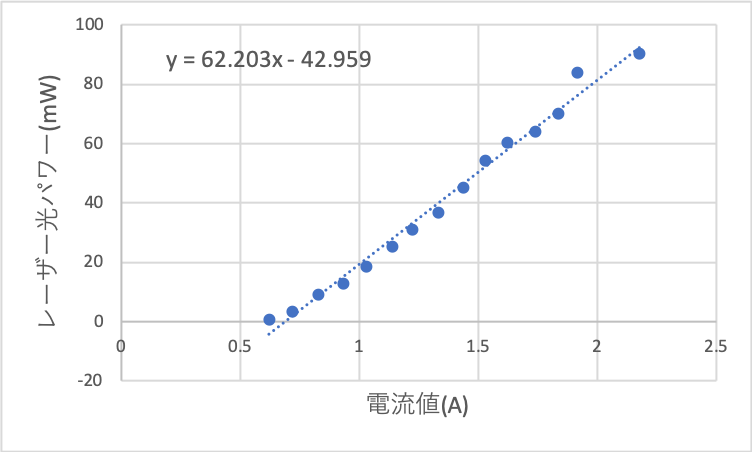
\includegraphics[width=0.8\linewidth]{fig3.png}
 \end{center}
 \caption{検量線}
 \label{fig:3}
\end{figure}

\subsection{考察}
まずレーザートラッピングの原理について考える.
対物レンズでポリスチレン球にレーザー光を集光した時レーザーの光路は図\ref{fig:1-2}のようになる.
ポリスチレン球の周りの媒質が水なのでポリスチレン球に入ったレーザー光はスネルの法則に従って屈折して透過することになるがこの時ポリスチレン球は屈折した光によって反作用が働きF1,F2のような力積を受ける.
それぞれの合力を考えるとFのようになるためレーザーの放射圧とつり合う箇所でポリスチレン球は水中で静止することができる.
同様にレーザー光がつりあいの位置から微小に左右にずれた際にも焦点位置に向かって反作用により力が働くためにレーザー光にトラップされたようにポリスチレン球が捕捉されることとなる.
レーザー光がポリスチレン球に入った瞬間にレーザー光に引き寄せられたのは球がレーザーから力を受ける際に図\ref{fig:1-2}のように安定の状態を取ろうとした結果であると考えられる.

また,この現象はポリスチレン球の屈折率が溶媒よりも大きい時に起こり溶媒よりも屈折率が小さくなると屈折の反作用が反発力となって働きトラップすることができなくなると予想される.
さらに金属のように反射率が高い物質に対しても屈折よりも反射による反作用の寄与が大きくなることによって力がつり合わずトラップできないと予想される.
したがって今回の実験ではレーザー集光の分解能を上げるために油侵レンズを使うなどの方法が考えられるが,その場合ポリスチレン球と媒質との屈折率が等しくなりトラップできなくなると考えられる.

次にレーザー駆動電流とレーザー光強度の関係については図\ref{fig:3}より概ね比例関係があると考えられる.
そこで二つの値は最小二乗法によって求めた数式y=62.203x+42.959の関係に従うと考えられる.
ここでデータのばらつきが生じたのはレーザー駆動電流が安定せず測定途中に上昇してしまったことが考えられる.
特に2A付近では安定した値を示さなかったので実際の値よりも大きい値を観測してしまった可能性が高い.

さらにポリスチレン球に焦点を合わせた際にレーザーの集光スポットが広がったのはポリスチレン球がガラスディッシュよりも上に位置しているためにポリスチレン球に焦点が合う位置ではガラスの底で反射された光はある程度の広がりを持ってしまうためだと考えられる.

\begin{figure}[htbp]
 \begin{center}
  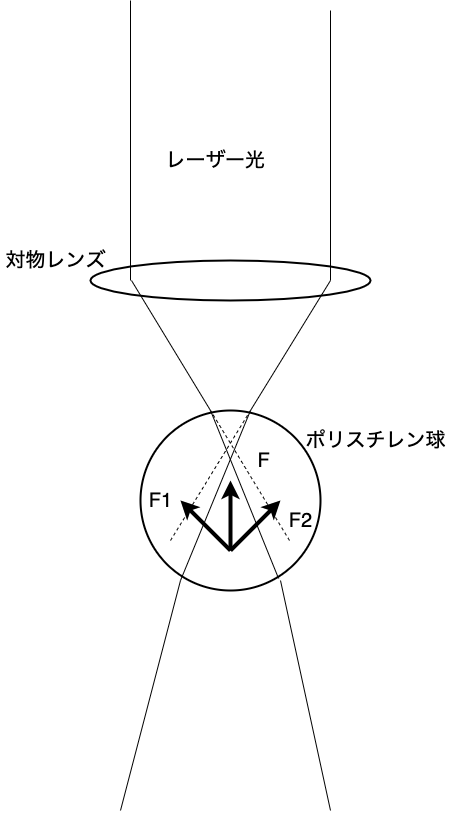
\includegraphics[width=0.8\linewidth]{fig1-2.png}
 \end{center}
 \caption{トラッピング原理}
 \label{fig:1-2}
\end{figure}


%=============================================================
\newpage
\end{document}
